\documentclass[12pt,a4paper]{report}
\usepackage[utf8]{vietnam}
\usepackage{amsmath}
\usepackage{amsfonts}
\usepackage{amssymb}
\usepackage{makeidx}
\usepackage{graphicx}
\usepackage{fancybox}
\usepackage[left=3.50cm, right=2.00cm, top=3.50cm, bottom=3.00cm]{geometry}
\usepackage{scrextend}
\changefontsizes{13pt}
\usepackage{fancyhdr}
\pagestyle{fancy}
\lhead{\textit{Tìm hiểu framework VueJS}}
\chead{}
\rhead{\textit{GVHD: TS Lê Hải Hà}}
\lfoot{\textit{SVTH: Hoàng Thanh Lưu}}
\cfoot{\thepage}
\rfoot{\textit{Toán Tin K61}}
\renewcommand{\headrulewidth}{0.4pt}
\renewcommand{\footrulewidth}{0.4pt}
\begin{document}
	\thisfancypage{%đóng khung trang này
		\setlength{\fboxsep}{0pt}% 8pt là độ dày của đường viền
		\fbox}{} % phần nội dung sau là tương tự như đã làm
	\thispagestyle{empty}
	\begin{center}
		\vspace*{0.2cm}
		\fontsize{14}{12}
		\textbf{TRƯỜNG ĐẠI HỌC BÁCH KHOA HÀ NỘI}\\
		\textbf{VIỆN TOÁN ỨNG DỤNG VÀ TIN HỌC}\\
		\textbf{------ o0o ------}
	\end{center}
	\vspace*{0.8cm}
	\begin{center}
		
\includegraphics[scale=.5]{bk.png}
	\end{center}
	\vspace*{0.8cm}
	\begin{center}
		\fontsize{20}{18}
		\textbf{THỰC TẬP KĨ THUẬT}\\
		\vspace*{0.8cm}
		\fontsize{18}{16}
		\textbf{TÌM HIỂU FRAMEWORK VUEJS}\\
		\fontsize{14}{16}
		\textbf{Chuyên ngành: Toán Tin}
	\end{center}
	\vspace*{0.7cm}
	\begin{center}
		\fontsize{14}{16}
		\begin{tabular}{ll}
			
			\textbf{Giảng viên hướng dẫn:} & \textbf{TS Lê Hải Hà} \\ 
			\textbf{Sinh viên thực hiện:} & \textbf{Hoàng Thanh Lưu} \\ 
			\textbf{Mã số sinh viên:} & \textbf{20162602}\\
			\textbf{Lớp:}  & \textbf{Toán Tin K61} \\ 
		\end{tabular} \\
		\vspace*{2.7cm}
		\fontsize{14}{16}
		\textbf{Hà Nội - 7/2020}
	\end{center}
	
	\chapter*{Lời nói đầu}
	Trong thời đại công nghệ thông tin ngày càng phát triển nhanh và mạnh mẽ như hiện nay
	các phần mềm ứng dụng, trang web trực tuyến cũng không ngừng phát triển nhằm phục vụ các yêu cầu của người dùng. Xây dựng một trang web cơ bản không chỉ đáp ứng những yêu cầu, tính năng cơ bản về chức năng nghiệp vụ mà còn cần đáp ứng về mặt đẹp mắt, thân thiện, tối ưu hóa trải nghiệm người dùng. Front End là cách gọi quy trình sử dụng các ngôn ngữ HTML, CSS, JavaScript thiết kế và xây dựng giao diện cho các trang web hoặc ứng dụng web để người dùng có thể xem và tương tác trực tiếp trên đó.\\\\
	Mục tiêu của việc thiết kế trang web là giúp cho người dùng dễ dàng sử dụng khi mở trang web. Điều này rất khó khăn vì trong thực tế người dụng sử dụng rất nhiều loại thiết bị khác nhau với kích thước và độ phân giải khác nhau, do đó buộc Front End Developer phải xem xét hết các khía cạnh này khi thiết kế trang web. Cần phải đảm bảo trang web xuất hiện chính xác trên các trình duyệt khác nhau, hệ điều hành khác nhau và các thiết bị khác nhau.\\\\
	Trong khuôn khổ nội dung thực tập, em được giao nhiệm vụ nghiên cứu về một framework có tuổi đời khá trẻ và ngày càng được sử dụng nhiều, và hiện tại đang được sử dụng để xây dựng giao diện web tròn các dự án tại công ty Skymap, đó là VueJS.\\\\
	Để có được báo cáo thực tập này em xin được gửi lời cảm ơn chân thành nhất tới Ban
	lãnh đạo, các phòng ban của công ty Skymap đã tạo điều kiện thuận lợi cho em được
	tìm hiểu, học tập, tiếp thu được những kiến thức thực tiễn trong suốt quá trình thực
	tập tại công ty.\\\\Cuối cùng em xin chân thành cảm ơn các thầy cô trong Viện toán ứng dụng và tin học
	đã trang bị cho em những kiến thức quý báu trong suốt thời gian học tập vừa qua, qua
	đó em có thể vận dụng các kiến thức đã học được trong thời gian thực tập tại công ty,
	để rồi có thêm được nhiều kiến thức thực tế và hoàn thành tốt quá trình thực tập.
	
	\tableofcontents
\chapter{Khái quát về công ty Skymap}
\section{Giới thiệu về công ty}
Công ty Trách nhiệm hữu hạn Công nghệ cao Skymap (Skymap Việt Nam) là chi nhánh của
công ty Skymap Global Singapore. Công ty gồm gần 50 nhân viên chính thức trong
đó TS. Lê Hải Hà hiện giữ chức vụ giám đốc công ty. Hiện tại công ty đang phát
triển các lĩnh vực hoạt động chính như sau:
\subsection{Mảng phát triển giải pháp công nghệ thông tin doanh nghiệp}
Skymap có kinh nghiệm trong việc áp dụng công nghệ thông tin vào giải quyết các bài toán thực tế doanh nghiệp. Hiện công ty đang triển khai các sản phẩm hệ thống quản lý thông tin phục vụ doanh nghiệp:
\begin{itemize}
	\item Hệ thống quản lý lao động và hỗ trợ xây dựng hồ sơ thầu\\
	 Tên công ty: CÔNG TY CỔ PHẦN NƯỚC VÀ MÔI TRƯỜNG VIỆT NAM (VIWASE)\\ Thời gian triển khai: 2 tháng
	\item Hệ thống quản lý lao động và tiền lương\\
	Tên công ty: CÔNG TY CỔ PHẦN ĐẦU TƯ THẾ GIỚI SỮA. (MILK WORLD INVESTMENT JOINT STOCK COMPANY) \\Thời gian triển khai: 3 tháng
	\item Sản phẩm salestrekk 
	\\Salestrekk là hệ thống hỗ trợ bán hàng. Salestrekk là giải pháp quản lý quan hệ khách hàng, theo dõi và hỗ trợ hệ thống sale rep.
	Khách hàng chính của salestrekk là các công ty bán sản phẩm theo mô hình dự án cần theo dõi quá trình chăm sóc khách hàng, các công ty có hệ thống sale, nhân viên thị trường cần quản lý và hỗ trợ tạo đơn hàng với tổng công ty. \\\\
	Tính năng nổi bật của salestrekk là hệ thống bản đồ cho phép có cái nhìn trực quan về hệ thống sale, tình hình các vùng kinh doanh. Khả năng ghi lại vị trí của app di động cho phép quản lý sale và công việc chăm sóc khách hàng.\\\\
	Tích hợp AI trong phân tích email khách hàng để phân tích cảm xúc khách hàng.
	
	
	\item Sản phẩm ứng dụng chấm công thông minh\\Thay thế máy chấm công vân tay bằng giải pháp tiết kiệm chi phí – ứng dụng chấm công trên mobile. Giải quyết được bài toán chấm công, kết nối tự động với hệ thống tính lương.
\end{itemize}
\subsection{Mảng bản đồ}
Skymap Việt Nam là công ty đứng đầu về số hóa và khai thác các hệ thống
thông tin địa lý, các giải pháp toàn diện về xử lý thông tin liên quan đến dữ
liệu địa lý và xử lý bản đồ.\\\\
Các dự án đang triển khai: hệ thống thông tin cháy rừng, cổng thông tin rà phá
bom mìn quốc gia.

\subsection{Mảng Machine Learning}
Skymap Việt Nam hiện đang ứng dụng công nghệ machine learning và AI vào giải quyết các bài toán trích xuất thông tin từ ảnh vệ tinh. Các ứng dụng đang phát triển:
\begin{itemize}
	\item Road detection: Nhận dạng đường từ ảnh vệ tinh.
	\item Building footprint: Vẽ móng các tòa nhà từ ảnh vệ tinh. Tiền đề cho phát triển bản đồ thành phố 3D.
	\item Tree couting: Đếm số lượng cây từ ảnh vệ tinh. Theo dõi số lượng cây trên diện tích rừng cho các công ty trồng cọ lấy dầu giúp đếm chính xác đến 95\% số lượng cây cọ, phân loại cây cọ chỉ bằng ảnh máy bay không người lái (UAV).
\end{itemize}

\section{Lịch sử phát triển}
Công ty TNHH công nghệ cao Skymap (Skymap Việt Nam) được thành lập vào ngày 25/01/2017, là chi nhánh của công ty Skymap Global Singapore với ngành nghề chính là nghiên cứu và phát triển phần mềm. \\\\ Trong bối cảnh số hóa toàn cầu, xu hướng phát triển mạnh mẽ của internet, các tổ chức doanh nghiệp muốn lựa chọn những giải pháp tối ưu nhất cho việc quản lý thông tin doanh nghiệp. Chính vì đó Skymap được ra đời nằm đáp ứng các nhu cầu số hóa, quản lý thông tin doanh nghiệp với chất lượng sản phẩm tốt nhất và giá cả cạnh tranh nhất tại Hà Nội. \\\\ Trong quá trình phát triển, Skymap luôn ý thức được việc giữ gìn giá trị thương hiệu mình đã xây dựng, không ngừng hoàn thiện để khách hàng luôn đặt niềm tin vào những sản phẩm của công ty và gắn bó với Skymap như một người bạn đáng tin cậy.

\section{Phương châm công ty}
\textit{Mỗi khó khăn mà doanh nghiệp Việt đang gặp phải là một bài toán mà công ty Trách nhiệm hữu hạn công nghệ cao Skymap đang từng ngày giải quyết.}\\\\
\textit{Nụ cười của doanh nghiệp là niềm vui và niềm tự hào của Skymap khi mang tới những giải pháp công nghệ tốt nhất, hoàn thiện nhất, nhanh nhất.}

\chapter{Quá trình thực tập}
\section{Các công việc được giao trong quá trình thực tập}
\begin{itemize}
	\item Tìm hiểu về framework VueJS
	\item Xây dựng ứng dụng nhỏ demo 
\end{itemize}
\section{Một số kiến thức cơ bản về VueJS}
\subsection{Giới thiệu về VueJS}
\begin{center}
	
\includegraphics[scale=.8]{1}
\end{center}
\subsubsection{Lịch sử hình thành và phát triển}
\begin{itemize}
	\item Vue được tạo bởi Evan You sau khi làm việc ở Google, khi đó Evan đang dùng AngularJS cho một số dự án, và Evan nói rằng: "Tôi tưởng tượng, điều gì sẽ xảy ra nếu tôi trích một phần mà tôi thực sự thích về Angular và xây dựng một cái gì đó nhẹ nhàng mà không cần thêm các khái niệm bổ sung?".Vue ban đầu được phát hành lần đầu vào tháng 2 năm 2014. Dự án này đã được đăng lên HackerNew, Echo Js trong ngày đầu ra mắt.
	\item Hiện tại, số lượng "thích" (star) trên Github cho dự án của Vue đang ngày càng tăng nhanh. Vuejs là một trong những project phổ biến nhất trên Github và thứ 2 trong số các JavaScript Framework (chỉ sau React), Vue đã vượt qua các thư viện / framework nổi tiếng khác như Angular 1.x, JQuery, Backbonejs,...
\end{itemize}
\subsubsection{VueJS là gì?}
Vue.js, gọi tắt là Vue, là một framework linh động dùng để xây dựng giao diện người dùng (user interfaces - UI). Khác với các framework nguyên khối, Vue được thiết kế từ đầu theo hướng cho phép và khuyến khích việc phát triển ứng dụng theo các bước. Khi phát triển lớp giao diện, người dùng chỉ cần dùng thư viện lõi (core library) của Vue, vốn rất dễ học và tích hợp với các thư viện hoặc dự án có sẵn. Cùng lúc đó, nếu kết hợp với những kĩ thuật hiện đại như SFC (single file components) và các thư viện hỗ trợ, Vue cũng đáp ứng được dễ dàng nhu cầu xây dựng những ứng dụng đơn trang (SPA - Single Page Applications) với độ phức tạp cao.

\subsubsection{VueJS với một số framework JS khác:}
\begin{center}
	
\includegraphics[scale=.8]{2}
\end{center}
Mức độ đánh giá (Theo diễn đàn github):
\begin{center}
	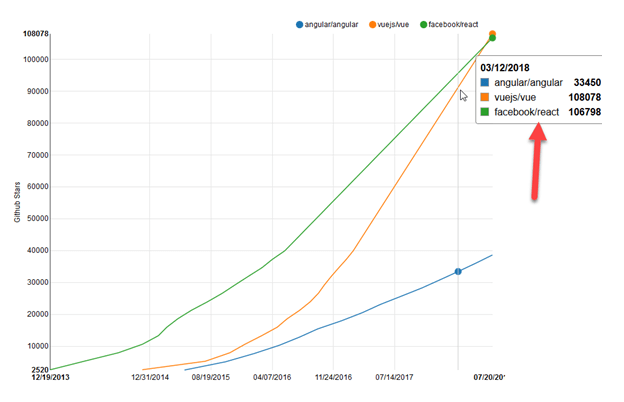
\includegraphics[scale=.7]{3}
\end{center}
Mức độ tìm hiểu:
\begin{center}
	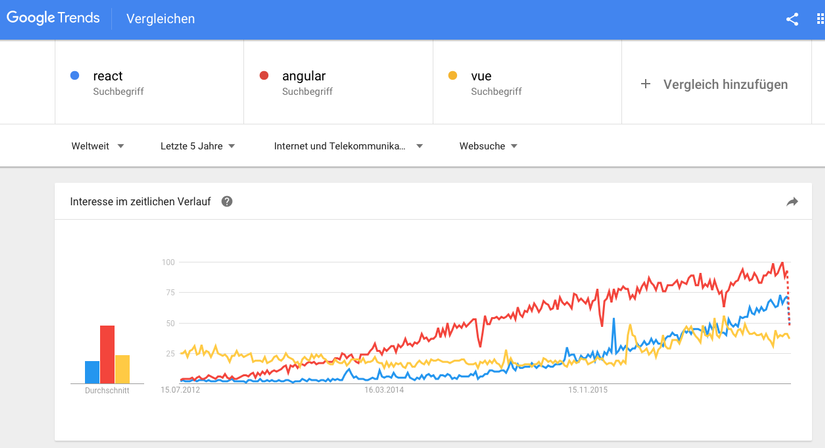
\includegraphics[scale=.52]{4}
\end{center}
Số lượt tải xuống:
\begin{center}
	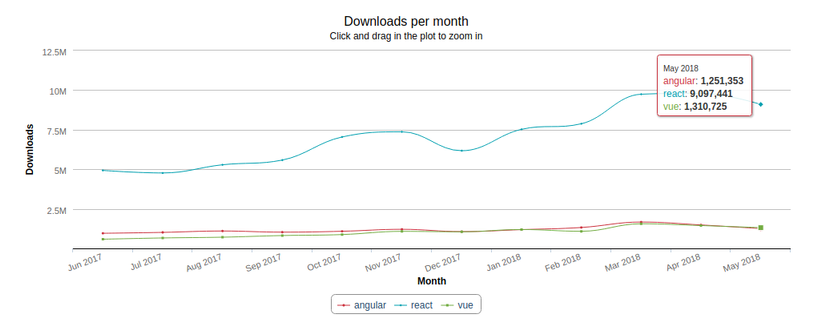
\includegraphics[scale=.55]{5}
\end{center}
\subsubsection{Ưu điểm}
 \begin{itemize}
		\item HTML được cấp quyền. Điều này có nghĩa rằng Vue.js có nhiều đặc điểm tương tự với Angular và điều này có thể giúp tối ưu hóa các khối HTML xử lý với việc sử dụng các components khác nhau.
		\item Tài liệu chi tiết. Vue.js có tài liệu hướng dẫn rất có khả năng có thể làm cho đường cong học tập trở nên nhanh hơn và tiết kiệm rất nhiều thời gian để phát triển một ứng dụng chỉ sử dụng kiến thức cơ bản về HTML và JavaScript.
		\item 	Khả năng thích ứng. Nó cung cấp một khoảng thời gian chuyển đổi nhanh từ các khung công tác khác sang Vue.js do sự tương tự với Angular và React về mặt thiết kế và kiến trúc.
		\item 	Tích hợp tuyệt vời. Vue.js có thể được sử dụng cho cả ứng dụng xây dựng một trang và giao diện web khó hơn của ứng dụng. Điều chính là các bộ phận tương tác nhỏ hơn có thể dễ dàng tích hợp vào cơ sở hạ tầng hiện tại mà không có tác động tiêu cực đến toàn bộ hệ thống.
		\item 	Large scaling (Chia tỷ lệ lớn). Vue.js có thể giúp phát triển các mẫu tái sử dụng khá lớn có thể được tạo ra mà không có thêm thời gian được phân bổ cho điều đó theo cấu trúc đơn giản của nó.
		\item 	Kích thước nhỏ. Vue.js có thể có trọng lượng khoảng 20KB giữ tốc độ và tính linh hoạt cho phép đạt hiệu suất tốt hơn nhiều so với các khung công tác khác.
	\end{itemize}
\subsubsection{Nhược điểm}
\begin{itemize}
	\item Thiếu nguồn lực. Vue.js vẫn có thị phần khá nhỏ so với React hay Angular, có nghĩa là chia sẻ tri thức trong framework này vẫn còn trong giai đoạn đầu.
	\item Rủi ro về tính linh hoạt. Đôi khi, Vue.js có thể có vấn đề trong khi tích hợp vào các dự án lớn và vẫn không có kinh nghiệm với các giải pháp có thể, nhưng họ chắc chắn sẽ đến sớm.
	\item Thiếu tài liệu tiếng Anh đầy đủ. Điều này dẫn đến một phần phức tạp trên một số giai đoạn phát triển, tuy nhiên, ngày càng có nhiều tài liệu được dịch sang tiếng Anh.
\end{itemize}
\subsubsection{Sử dụng}
Các công ty sử dụng Vue.js: Xiaomi, Alibaba, WizzAir, EuroNews, Grammarly, Gitlab và Laracasts, Adobe, Behance, Codeship, Reuters.

\subsection{Bắt đầu}
Chỉ cần tải file thư viện về rồi sử dụng nó trong thẻ script. Vue sẽ được đăng ký thành một biến toàn cục.\\\\
Các bản: Development với đầy đủ chế độ cảnh báo, Debug, bảng Production không có các cảnh báo, nhẹ hơn, file zip.\\\\
Cách sử dụng đơn giản nhất: Copy đoạn mã nguồn sau cho vào project:
\begin{center}
	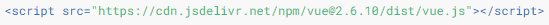
\includegraphics[scale=.8]{6}
\end{center}
Hoặc có thể cài đặt thông qua npm: \$ npm install vue
\subsection{Đối tượng Vue}
\subsubsection{Tạo một đối tượng Vue}
Một ứng dụng Vue luôn được bắt đầu bằng cách khởi tạo một đối tượng Vue (Vue instance) sử dụng hàm Vue:\\
	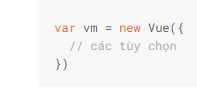
\includegraphics[scale=1]{7}
\\Khi khởi tạo một đối tượng Vue, chúng ta truyền vào một object options với các tùy chọn. Một component Vue cũng là một đối tượng Vue và do đó cũng nhận cùng một object options (trừ một số tùy chọn chỉ dành riêng cho root). \subsubsection{Dữ liệu và phương thức} Khi một đối tượng Vue được khởi tạo, tất cả các thuộc tính (property) được tìm thấy trong object data sẽ được thêm vào reactivity system (hiểu nôm na là “hệ thống phản ứng”) của Vue. Điều này có nghĩa là view sẽ “react” (phản ứng) khi giá trị của các thuộc tính này thay đổi, và tự cập nhật tương ứng với các giá trị mới.\\
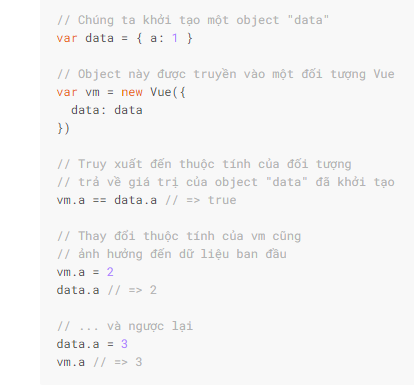
\includegraphics[scale=1]{8}\\Khi dữ liệu thay đổi, view sẽ render lại. Cũng nên lưu ý rằng một thuộc tính trong object data chỉ trở nên reactive nếu nó đã tồn tại khi chúng ta khởi tạo đối tượng Vue.\subsubsection{Vòng đời đối tượng} Khi được khởi tạo, một đối tượng Vue sẽ đi qua nhiều bước khác nhau - cài đặt quan sát dữ liệu (data observation), biên dịch template, gắn kết vào DOM, cập nhật DOM khi dữ liệu thay đổi v.v. Trong suốt tiến trình này, nó cũng sẽ thực thi một số hàm gọi là lifecycle hook, giúp người dùng thêm code của mình vào các giai đoạn (stage) cụ thể trong vòng đời của đối tượng. 
\subsection{Cú pháp Template}
Vue.js sử dụng một cú pháp template dựa trên HTML, cho phép bạn ràng buộc (bind) một cách minh bạch cấu trúc DOM được render với dữ liệu của đối tượng Vue bên dưới. Tất cả các template của Vue đều là code HTML hợp lệ và có thể được parse bởi các trình duyệt và parser chuẩn. \\\\ Bên dưới, Vue biên dịch template thành các hàm render Virtual DOM (DOM ảo). Kết hợp với hệ thống reactivity (phản ứng), Vue có thể xác định một cách thông minh số lượng tối thiểu các component cần phải render lại, và áp dụng số lượng tối thiểu các hiệu chỉnh về DOM khi trạng thái của ứng dụng thay đổi. 
\subsubsection{Văn bản}
Hình thức ràng buộc dữ liệu cơ bản nhất là nội suy văn bản (text interpolation) sử dụng cú pháp “mustache” (“ria mép” – hai dấu ngoặc nhọn):\\
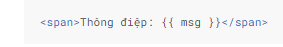
\includegraphics[scale=1]{10}\\Thẻ mustache sẽ được thay thế bằng giá trị của thuộc tính msg trên object data tương ứng, và cũng sẽ được cập nhật bất cứ khi nào thuộc tính này thay đổi.
\subsubsection{HTML thuần túy}
Cú pháp mustache sẽ thông dịch dữ liệu ra thành văn bản thuần túy (plain text), nghĩa là các kí tự HTML đặc biệt như <>\&"' sẽ được mã hóa. Để xuất ra HTML thuần túy, bạn sẽ cần đến directive v-html.\\
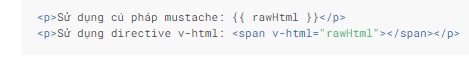
\includegraphics[scale=1]{11}
\subsubsection{Các thuộc tính HTML}
Cú pháp mustache không dùng được bên trong các thuộc tính HTML. Thay vào đó, bạn hãy dùng directive v-bind:
\\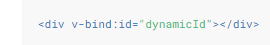
\includegraphics[scale=1]{12}\\Directive này cũng hoạt động với các thuộc tính boolean như disabled và selected - các thuộc tính này sẽ được bỏ đi khi biểu thức được tính toán trả về kết quả sai (falsy).
\subsubsection{Sử dụng biểu thức Javascript}
Cho đến nay chúng ta chỉ mới bind vào các khóa thuộc tính dơn giản trong template. Tuy nhiên, thật ra Vue hỗ trợ sức mạnh toàn diện của các biểu thức JavaScript bên trong toàn bộ các ràng buộc dữ liệu (data binding):\\
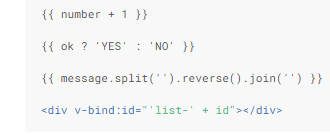
\includegraphics[scale=1]{13}
\subsubsection{Directive}
Directive là các thuộc tính đặc biệt với prefix (tiếp đầu ngữ) v-. Giá trị của thuộc tính directive phải là một biểu thức JavaScript đơn lẻ (ngoại trừ v-for mà chúng ta sẽ đề cập sau). Nhiệm vụ của một directive là áp dụng các hiệu ứng phụ vào DOM khi giá trị của biểu thức thay đổi.
\subsubsection{Tham số}
Một số directive có thể nhận vào một tham số, đánh dấu bằng một dấu hai chấm theo sau tên của directive. Ví dụ, directive v-bind được dùng để cập nhật động một thuộc tính HTML:\\
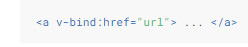
\includegraphics[scale=1]{14}\\Ở đây href là tham số hướng dẫn directive v-bind ràng buộc thuộc tính href vào giá trị của biểu thức url.
\subsubsection{Modifier}
Modifier là các hậu tố (postfix) đặc biệt được đánh dấu bằng một dấu chấm, chỉ rõ rằng một directive phải được ràng buộc theo một cách đặc biệt nào đó. Ví dụ, modifier .prevent hướng dẫn directive v-on gọi event.preventDefault() khi sự kiện được kích hoạt:\\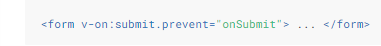
\includegraphics[scale=1]{15}
\subsubsection{Cú pháp rút gọn}
Prefix v- đóng vai trò gợi ý trực quan để nhận ra các thuộc tính riêng của Vue trong template. Điều này có ích khi bạn sử dụng Vue vào các dự án có sẵn, tuy nhiên đối với các directive được dùng thường xuyên thì v- có thể trông hơi rườm rà. Thêm vào đó v- trở nên kém quan trọng hơn khi bạn xây dựng các ứng dụng một trang, trong đó Vue quản lí toàn bộ các template. Vì thế Vue cung cấp dạng rút gọn (shorthand) đặc biệt cho hai trong số các directive được dùng nhiều nhất, v-bind và v-on:\\
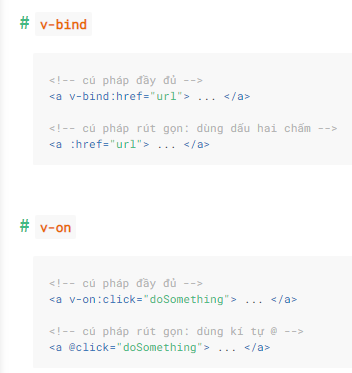
\includegraphics[scale=1]{16}
\subsection{Computed property và watcher}
\subsubsection{Computed property}
Viết biểu thức trực tiếp trong template rất tiện, nhưng chỉ dành cho những biểu thức có tính toán đơn giản. Những biểu thức phức tạp được viết theo cách đó sẽ khiến template cồng kềnh và khó bảo trì. Đó là lí do tại sao đối với bất kì logic nào phức tạp, bạn nên sử dụng computed property. Ví dụ:
\\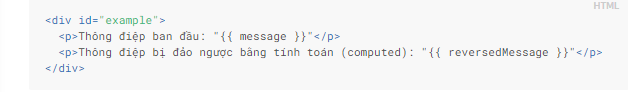
\includegraphics[scale=.93]{17}\\
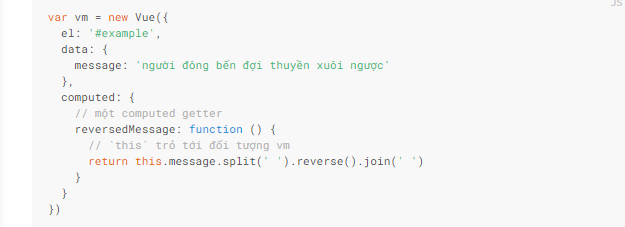
\includegraphics[scale=.93]{18}\\ Kết quả là: \\

\includegraphics[scale=.93]{19}\\Bạn có thể ràng buộc dữ liệu (data-bind) cho computed property trong template một cách bình thường như những thuộc tính khác. Vue biết được vm.reversedMessage phụ thuộc vào vm.message nên sẽ cập nhật bất kì ràng buộc (binding) nào phụ thuộc vào vm.reversedMessage khi vm.message thay đổi. Điểm hay nhất ở đây là chúng ta tạo ra được mối liên hệ giữa các thành phần phụ thuộc (dependency): các hàm getter của computed thì không bị hiệu ứng phụ (side effect), chính điều đó giúp dễ hiểu và dễ kiểm tra.
\subsubsection{Computed caching và phương thức}
Bạn có lẽ đã nhận ra chúng ta cũng có thể đạt được cùng một kết quả bằng cách sử dụng một phương thức:\\
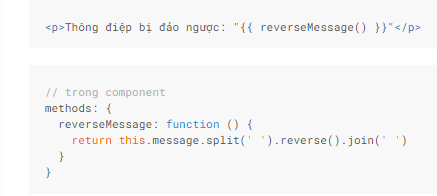
\includegraphics[scale=1]{20}\\Thay vì sử dụng computed property, chúng ta cũng có thể dùng một phương thức thay thế. Nếu xét về kết quả cuối cùng thì hai cách tiếp cận này thât ra chỉ là một. Tuy nhiên, sự khác biệt ở đây là computed property được cache lại dựa vào những những thành phần phụ thuộc (dependency). Một computed property chỉ được tính toán lại khi những thành phần phụ thuộc của chúng thay đổi. Điều này có nghĩa: miễn là giá trị của message không thay đổi, thì những truy cập tới computed reversedMessage sẽ ngay lập tức trả về kết quả được tính toán trước đó mà không phải chạy lại hàm một lần nữa.\\\\Để so sánh, một phương phương thức luôn được gọi khi có một sự kiện render lại (re-render) xảy ra.\\\\Tại sao chúng ta lại cần phải cache? Thử tưởng tượng chúng ta có một computed property A có nhiều thao tác tính toán trên một mảng dữ liệu lớn. Chúng ta lại có nhiều computed property phụ thuộc vào A. Nếu không cache lại, chúng ta phải thực thi hàm getter của A nhiều hơn mức cần thiết rất nhiều! Trong trường hợp bạn không muốn cache, hãy sử dụng một phương thức thay thế.
\subsubsection{Watcher}Computed property thích hợp cho hầu hết các trường hợp, nhưng cũng có lúc cần tới những watcher tùy biến. Đó là lí do tại sao Vue cung cấp một cách khái quát hơn để phản ứng lại với việc thay đổi dữ liệu trong watch. Cách sử dụng này rất hữu ích khi bạn muốn thực hiện những tính toán không đồng bộ và tốn kém liên quan đến việc thay đổi dữ liệu.\\\\ Ngoài tùy chọn watch, bạn cũng có thể sử dụng vm.\$watch API.

\subsection{Binding cho class và style}
\subsubsection{Binding cho class trong HTML}
Sử dụng cú pháp Object:\\Ta có thể truyền một object vào v-bind:class để bật tắt class một cách linh hoạt:\\
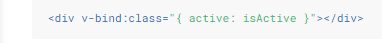
\includegraphics[scale=1]{21}
\\Cú pháp như trên nghĩa là class active sẽ được áp dụng tùy theo tính đúng sai (truthiness) của thuộc tính dữ liệu isActive.\\\\Bạn có thể bật tắt nhiều class bằng cách dùng nhiều field (trường) trong object. Thêm vào đó, directive v-bind:class và thuộc tính class thông thường có thể được dùng cùng lúc với nhau. Nếu chúng ta có template sau:\\
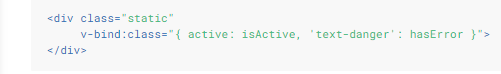
\includegraphics[scale=1]{22}\\ và dữ liệu truyền vào như thế này\\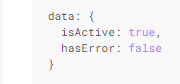
\includegraphics[scale=1]{23}\\ thì kết quả render sẽ là: \\
\includegraphics[scale=1]{24}\\Khi giá trị isActive hoặc hasError thay đổi, danh sách class sẽ được cập nhật tương ứng. Ví dụ, nếu hasError trở thành true, danh sách class sẽ trở thành "static active text-danger".
\\Object được bind cũng không bắt buộc phải khai báo trong template:\\
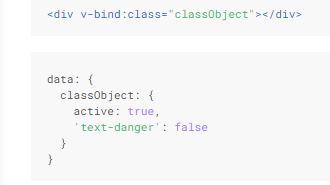
\includegraphics[scale=1]{25}\\Ví dụ trên sẽ render ra cùng một kết quả. Chúng ta cũng có thể bind vào một computed property (thuộc tính được tính toán) trả về một object. Dưới đây là một ví dụ điển hình cho kĩ thuật này:\\
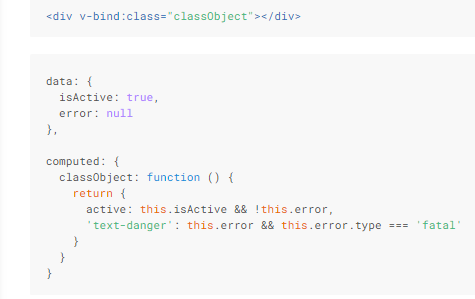
\includegraphics[scale=1]{26}\\
Sử dụng cú pháp mảng:\\\\Chúng ta có thể truyền một mảng vào v-bind:class để áp dụng một danh sách class:\\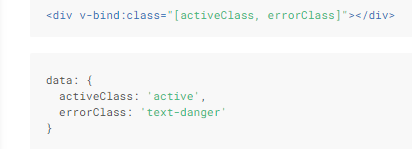
\includegraphics[scale=1]{27}\\ sẽ render ra kết quả sau:\\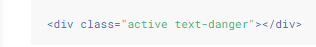
\includegraphics[scale=1]{28}\\Nếu muốn bật tắt theo điều kiện một class trong danh sách, bạn có thể dùng một toán tử ba ngôi (ternary expression):\\
\includegraphics[scale=1]{29}\\Đoạn code trên sẽ luôn luôn áp dụng class errorClass, nhưng chỉ áp dụng activeClass khi isActive mang giá trị đúng.\\\\Cách làm này có thể hơi dài dòng nếu bạn có nhiều class theo điều kiện. Do đó, bạn có thể dùng cú pháp object bên trong cú pháp mảng, như sau:\\
\includegraphics[scale=1]{30}
\subsubsection{Binding cho inline style}
Sử dụng cú pháp object: \\\\Cú pháp object của v-bind:style rất đơn giản - trông giống như CSS thông thường, chỉ khác ở chỗ nó là một object JavaScript. Bạn có thể dùng camelCase hoặc kebab-case (đặt trong dấu nháy nếu là kebab-case) đối với tên thuộc tính CSS:\\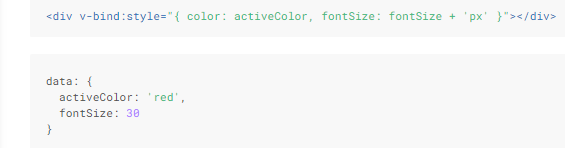
\includegraphics[scale=1]{31}\\
Thông thường thì ta nên bind vào một object dành riêng cho style để template được gọn gàng hơn: \\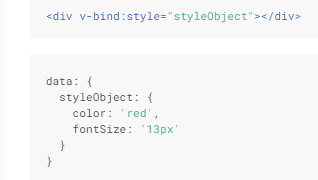
\includegraphics[scale=1]{32}\\Một lần nữa, cú pháp object thường được dùng kết hợp với các computed property trả về object.\\Sử dụng cú pháp mảng:\\\\Cú pháp mảng của v-bind:style giúp bạn áp dụng nhiều object style cho cùng một phần tử web:\\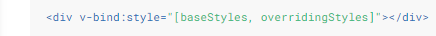
\includegraphics[scale=1]{33}\\ Tự động theeo Prefix:\\\\Khi bạn sử dụng một thuộc tính CSS còn khá mới và cần vendor prefix trong v-bind:style, ví dụ transform, Vue sẽ tự động phát hiện và thêm prefix thích hợp vào các style được áp dụng.\\\\Nhiều giá trị: \\\\Có thể cung cấp một mảng các giá trị (đã có prefix) cho một thuộc tính CSS, như sau:\\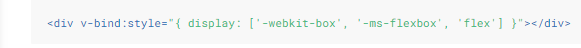
\includegraphics[scale=1]{34}\\Với kĩ thuật này, Vue sẽ chỉ render ra giá trị cuối cùng trong mảng mà trình duyệt hỗ trợ. Trong ví dụ trên, Vue sẽ render display: flex trên các trình duyệt hỗ trợ flexbox.
\subsection{Render theo điều kiện}
\subsubsection{v-if}
Trong các thư viện biên dịch template như Handlebars, thông thường chúng ta sẽ viết các khối điều kiện (conditional block) như sau:\\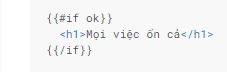
\includegraphics[scale=1]{35}\\Để làm điều này với Vue, chúng ta sử dụng directive v-if:\\
\includegraphics[scale=1]{36}\\Chúng ta cũng có thể thêm khối “else” bằng v-else:\\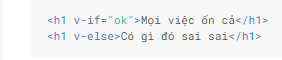
\includegraphics[scale=1]{37}\\Nhóm điều kiện với v-if trên thẻ <template>: Vì là một directive, v-if phải được dùng trên một phần tử đơn lẻ (single element) như <p> hoặc <div>. Nếu chúng ta muốn bật tắt một nhóm các phần tử thì sao? Chỉ cần dùng v-if trên một phần tử <template> với vai trò wrap (bọc) các phần tử lại thành một nhóm. Kết quả render cuối cùng sẽ không có phần tử <template> này.
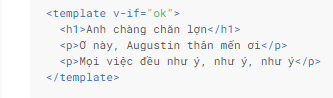
\includegraphics[scale=1]{38}\\Directive v-else-if đóng vai trò một khối “else if” cho v-if. Directive này có thể được dùng nhiều lần nối tiếp nhau:\\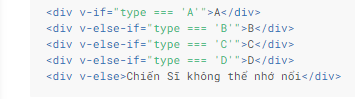
\includegraphics[scale=1]{39}\\Tương tự với v-else, phần tử với v-else-if phải theo ngay sau một phần tử v-if hoặc v-else-if.
\subsubsection{v-show}
Một lựa chọn nữa cho việc hiện hoặc ẩn một phần tử web theo điều kiện là directive v-show. Cách dùng v-show cũng tương tự với v-if:\\
\includegraphics[scale=1]{40}\\Điểm khác biệt giữa v-show và v-if là phần tử được đánh dấu với v-show sẽ luôn luôn được render và chứa trong DOM; v-show chỉ bật tắt thuộc tính display của phần tử này.
\subsection{Render theo danh sách}
\subsubsection{Map một mảng thành các phần tử web với v-for}
Chúng ta có thể dùng directive v-for để render một danh sách các item dựa trên một mảng. Directive v-for đòi hỏi một cú pháp đặc biệt dưới dạng item in items, trong đó items là mảng dữ liệu nguồn và item trỏ đến phần tử mảng đang được duyệt đến:\\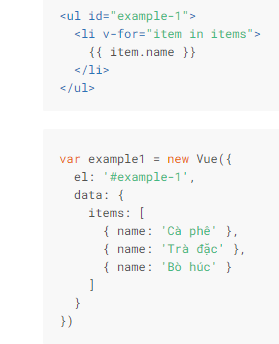
\includegraphics[scale=1]{41}\\Kết quả là \\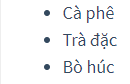
\includegraphics[scale=1]{42}\\Bên trong vòng lặp v-for chúng ta có toàn quyền truy xuất đến các thuộc tính của scope cha. v-for cũng hỗ trợ một tham số thứ hai (không bắt buộc) chỉ số thứ tự (index) của phần tử mảng hiện hành.\\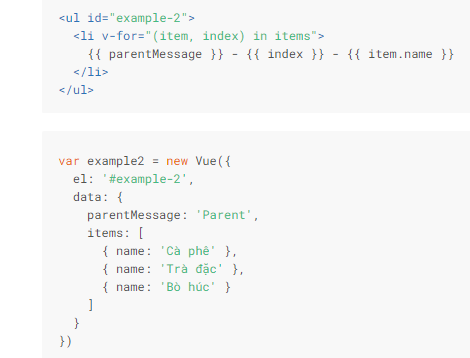
\includegraphics[scale=.95]{43}\\Kết quả là: \\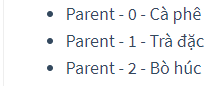
\includegraphics[scale=1]{44}\\Bạn cũng có thể dùng of để phân cách thay vì in. Cách này cũng gần hơn với cú pháp vòng lặp trong JavaScript.
\subsubsection{Dùng v-for với một object}Bạn cũng có thể dùng v-for để duyệt qua các thuộc tính của một object.\\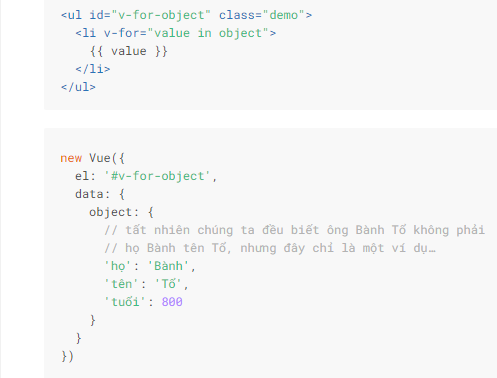
\includegraphics[scale=1]{45}\\Kết quả \\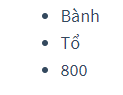
\includegraphics[scale=1]{46}\\Bạn cũng có thể cung cấp tham số thứ hai dùng cho khóa (key) của thuộc tính:\\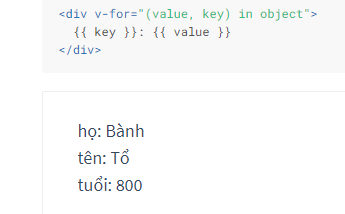
\includegraphics[scale=1]{47}
\subsubsection{Hiển thị kết quả đã được lọc hoặc sắp xếp}Đôi khi chúng ta muốn hiển thị một phiên bản đã được lọc (filter) hoặc sắp xếp (sort) của một mảng mà không thay đổi mảng đó. Trong trường hợp này, bạn có thể tạo một computed property trả về mảng đã được lọc hoặc sắp xếp. Ví dụ:\\
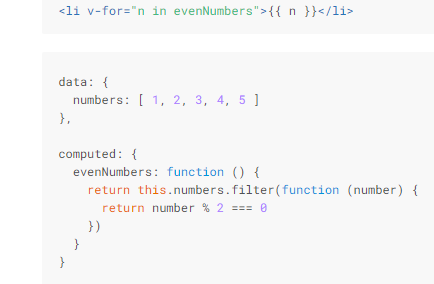
\includegraphics[scale=1]{48}\\Trong trường hợp không dùng được computed property (ví dụ trong các vòng lặp v-for), ta có thể dùng một phương thức: \\
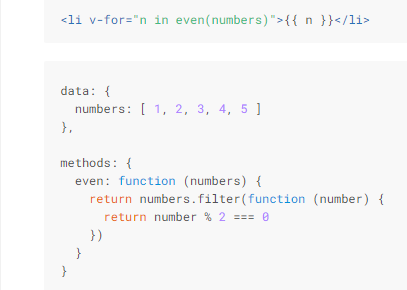
\includegraphics[scale=1]{49}
\subsubsection{v-for dùng với một dãy}
v-for cũng có thể nhận một số nguyên n. Trong trường hợp này, template sẽ được lặp lại n lần:
\\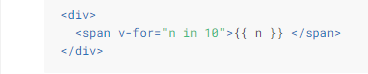
\includegraphics[scale=1]{50}\\Kết quả là: 1 2 3 4 5 6 7 8 9 10.
\subsubsection{v-for dùng với thẻ <template>} Tương tự với v-if, bạn có thể dùng v-for trên một thẻ <template> để render một lúc nhiều phần tử. Ví dụ: \\\includegraphics[scale=1]{51}
\subsubsection{v-for dùng với v-if}Khi được dùng trên dùng một node, v-for có độ ưu tiên cao hơn v-if, có nghĩa là v-if sẽ được thực thi một cách riêng biệt trên mỗi vòng lặp của v-for. Điều này có thể có ích khi bạn muốn render cho chỉ một số item, như trong ví dụ sau: \\\includegraphics[scale=1]{52}\\Ví dụ trên sẽ chỉ render những todo chưa hoàn thành.\\\\Ngược lại, nếu bạn muốn bỏ qua việc thực thi vòng lặp v-for theo điều kiện, hãy dùng v-if trên một phần tử wrapper (hoặc <template>). Ví dụ: \\\includegraphics[scale=1]{53}
\subsection{Xử lí sự kiện}
\subsubsection{Lắng nghe sự kiện} Chúng ta có thể dùng directive v-on để lắng nghe các sự kiện DOM và thực thi JavaScript khi những sự kiện này được kích hoạt. Ví dụ:\\\includegraphics[scale=1]{54}
\subsubsection{Phương thức xử lí sự kiện}Trong thực tế, logic để xử lí sự kiện thường phức tạp hơn, vì thế chứa JavaScript trực tiếp trong giá trị của thuộc tính v-on như trên là không khả thi. Đó là lí do v-on cũng có thể nhận tên của một phương thức mà bạn muốn gọi. Ví dụ:\\\includegraphics[scale=1]{55}
\subsubsection{Gọi phương thức inline} Thay vì bind trực tiếp tên phương thức, ta cũng có thể gọi phương thức trong một câu lệnh JavaScript:\\\includegraphics[scale=.95]{56}\\Đôi khi chúng ta cũng muốn truy xuất đến sự kiện DOM ban đầu từ câu lệnh JavaScript inline. Bạn có thể truyền sự kiện DOM vào phương thức thông qua biến \$event: \\\includegraphics[scale=1]{57}
\subsubsection{Event modifier}Trong rất nhiều trường hợp, chúng ta cần gọi event.preventDefault() hoặc là gọi\\ event.stopPropagation() bên trong một phương thức xử lí sự kiện. Tuy việc này không có gì khó, sẽ tốt hơn nếu các phương thức chỉ phải tập trung giải quyết logic dữ liệu thay vì cáng đáng các sự kiện DOM. Để giải quyết vấn đề này, Vue cung cấp các event modifier cho v-on. Event modfier là một hậu tố (postfix) cho directive, được biểu thị bằng một dấu chấm. \\".stop \quad .prevent \quad .capture \quad .self \quad .once"
\subsubsection{Key modifier} Khi lắng nghe các sự kiện bàn phím (keyboard event), chúng ta thường phải kiểm tra mã phím (key code). Vue hỗ trợ thêm key modifier (modifer cho mã phím) cho v-on trong các trường hợp này.
\subsubsection{Tại sao lại lắng nghe sự kiện trong HTML?} Bạn có thể lo ngại rằng toàn bộ việc lắng nghe sự kiện bằng cách đặt event listener trong HTML như thế này là vi phạm quy tắc “separation of concerns.” Cứ yên tâm, vì tất cả các hàm và biểu thức xử lí sự kiện của Vue được ràng buộc chặt chẽ với ViewModel, sẽ không có khó khăn gì trong việc bảo trì. Thật ra, sử dụng v-on còn có những lợi ích sau:
\begin{enumerate}
	\item Giúp định vị hàm xử lí trong code JavaScript được dễ dàng hơn bằng cách đọc lướt template HTML.
	\item Vì không phải attach hàm xử lí sự kiện trong JavaScript một cách thủ công, code trong ViewModel trở nên thuần logic và không phụ thuộc vào DOM. Điều này giúp chúng ta dễ viết test.
	\item Khi một ViewModel bị hủy, tất cả hàm xử lí sự kiện đính kèm cũng được tự động gỡ bỏ mà không cần bạn phải dọn dẹp.
\end{enumerate}
\subsection{Cơ bản về Component}
\subsubsection{Ví dụ cơ bản} Đây là ví dụ về một component trong Vue:
\\\includegraphics[scale=1]{58}\\Component là các đối tượng Vue có thể sử dụng lại được với một cái tên: trong trường hợp này là <button-counter>. Chúng ta có thể dùng component này như là một phần tử bên trong đối tượng Vue gốc được tạo bởi new Vue: \\\includegraphics[scale=1]{59}
\subsubsection{Tổ chức component}
Một ứng dụng thường được tổ chức dưới dạng một cây component lồng nhau: \begin{center}
	\includegraphics[scale=.7]{60}
\end{center} Để có thể được sử dụng trong các template, component phải được đăng kí. Có hai cách đăng kí component: toàn cục và cục bộ. Trên đây chúng ta chỉ mới đăng kí component ở cấp toàn cục với Vue.component: \\\includegraphics[scale=1]{61}\\Component đăng kí ở cấp toàn cục có thể được dùng trong template của bất kì đối tượng Vue gốc (new Vue) nào được tạo ra sau đó – và trong tất cả các component con trên cây component của đối tượng đó.
\subsubsection{Truyền dữ liệu xuống component con bằng prop} Prop là các thuộc tính tùy chỉnh mà bạn có thể đăng kí trên một component. Khi một giá trị được truyền vào một prop, nó trở thành một “\_prop\_erty” của đối tượng component đó. Để truyền tựa đề (title) vào component bài viết (blog-post), chúng ta sử dụng tùy chọn props: \\\includegraphics[scale=1]{62}\\Một component có thể có bao nhiêu prop tùy ý, và prop có thể nhận bất kì giá trị gì. Trong template trên đây, bạn có thể thấy là chúng ta có thể truy xuất giá trị này trên đối tượng component, giống như với data. Một khi prop đã được đăng kí, bạn có thể truyền dữ liệu vào như một thuộc tính tùy chỉnh, ví dụ: \\\includegraphics[scale=1]{63}\\Tuy nhiên, trong một ứng dụng điển hình, bạn có lẽ sẽ có một mảng các bài viết trong data: \\\includegraphics[scale=1]{64}\\và sau đó render một component cho mỗi bài viết: \\\includegraphics[scale=1]{65} \\Trên đây, bạn có thể thấy là chúng ta dùng v-bind để truyền động prop. Cách làm này đặc biệt hữu ích khi bạn không biết trước được chính xác nội dung bạn sẽ render, như khi lấy bài viết từ một API.
\subsubsection{Một phần tử gốc đơn lập}
Khi xây dựng component <blog-post> cho bài viết, thế nào rồi template của bạn cũng sẽ chứa nhiều thứ hơn là mỗi title. Ít nhất bạn cũng sẽ có thêm nội dung bài viết:\\\includegraphics[scale=1]{66}\\Nhưng nếu bạn sử dụng template này, Vue sẽ thông báo lỗi every component must have a single root element (mỗi component phải có một phần tử gốc đơn lập). Bạn có thể sửa lỗi này bằng cách bọc template trong một phần tử cha, ví dụ:\\\includegraphics[scale=1]{66}
\subsubsection{Component động}
Đôi khi bạn muốn chuyển qua lại giữa các component, ví dụ như trên một giao diện tab: \\\includegraphics[scale=1]{67}\\Ví dụ trên hoạt động nhờ thuộc tính đặc biệt is của một component trong Vue:\\\includegraphics[scale=1]{68}\\Trong ví dụ trên, currentTabComponent có thể chứa:\begin{itemize}
	\item tên của một component đã được đăng kí, hoặc
	\item object chứa các tùy chọn của một component
\end{itemize}
\section{Xây dựng  game xúc xắc sử dụng VueJS}
\subsubsection{Giao diện trang chủ} 
\begin{center}
	\includegraphics[scale=.42]{69}
\end{center}
\subsubsection{Giao diện người chơi} 
\begin{center}
	\includegraphics[scale=.42]{70}
\end{center}
\subsubsection{Giao diện người chiến thắng} 
\begin{center}
	\includegraphics[scale=.42]{71}
\end{center}
\subsubsection{Giao diện người thua cuộc} 
\begin{center}
	\includegraphics[scale=.42]{72}
\end{center}
\subsubsection{Giao diện luật chơi} 
\begin{center}
	\includegraphics[scale=.42]{73}
\end{center}
\chapter{Kết luận}
Trên đây là những kiến thức em tìm hiểu cũng như được học trong suốt thời gian thực
tập tại công ty. Sau gần 10 tuần thực tập tại công ty em đã có thêm được nhiều kĩ năng và kiến
thức nhất định về lập trình web, lập trình front-end sử dụng framework VueJS. Em cũng đã xây dựng được một ứng dụng nhỏ demo để vận dụng các kiến thức tìm hiểu được từ VueJS. \\\\Do thời gian tìm hiểu cũng như kiến thức còn hạn chế nên bài báo cáo
của em không tránh khỏi thiếu sót, em rất mong có được sự đóng góp chỉnh sửa từ
các thầy cô và anh chị để bài báo cáo của em được hoàn thiện hơn.\\\\ Em xin chân thành
cảm ơn.

\begin{thebibliography}{}
	\bibitem{latex} https://vi.wikipedia.org/wiki/Vue.js
	\bibitem{latex} https://vuejs.org/
	\bibitem{latex} https://viblo.asia/p/so-sanh-giua-reactjs-va-vuejs-va-angular-3Q75wdrQKWb
\end{thebibliography}
\end{document}